\chapter{Results}\label{ch:results}

This chapter reports four classes of empirical results in service of the central question of the thesis: whether gradient-based parameter estimation can produce useful parameter updates for the \gls{AdEx} model.
\Cref{sec:results:verification} establishes that the forward model is correct, by comparing our \texttt{Jaxley} \gls{AdEx} channel and its surrogate-gradient variant against Brian2 on three reference parameter sets;
this is a precondition for the rest of the chapter, since it rules out the possibility that any later failure is an artefact of the dynamics rather than a property of the optimisation.
\Cref{sec:results:landscape} characterises the loss surfaces the optimiser actually descends, on a $20\times 20$ two-parameter sweep over all $\binom{8}{2}=28$ trainable pairs for each of four differentiable losses, supplemented by focused panels that isolate one diagnostic feature per loss.
The picture is a thin spiking valley flanked by a large non-spiking plateau.
\Cref{sec:results:training} reports what happens when an optimiser is run on those surfaces: two worked examples (one synthetic, one on a real recording) and a recovery-radius benchmark over $2{,}700$ paired runs that compares three differentiable losses against two Nelder--Mead baselines on identical perturbed initialisations.

%%%%%%%%%%%%%%%%%%%%%%%%%%%%%%%%%%%%%%%%%%%%%%%%%%%%%%%%%%%%%%%%%%%%%%%%%%%%
\section{An AdEx Channel for Jaxley}\label{sec:results:verification}

The first concrete outcome of this thesis is a working \gls{AdEx} channel for \texttt{Jaxley}, validated against an established reference simulator.
Following the protocol of \cref{sec:method:adex:verification}, we compare our implementation to Brian2 \cite{Stimberg2019} on all three reference parameter sets from Naud et al.~\cite{Naud2008} --- tonic, adaptation and original --- which together cover the qualitatively distinct firing regimes \gls{AdEx} is meant to reproduce.

Across all three configurations, the two simulators produce identical spike counts, and the maximum pair-wise spike-timing difference stays below $1$\,ms.
\Cref{fig:brian_comparison} shows the side-by-side comparison of voltage traces, adaptation current $w$, and spike times.
The remaining sub-millisecond differences are what one would expect given that the two simulators use different integration schemes for the membrane equation, and they are well below the temporal resolution at which we later evaluate spike-timing accuracy via the coincidence factor $\Gamma$.

\begin{figure*}
  \begin{center}
    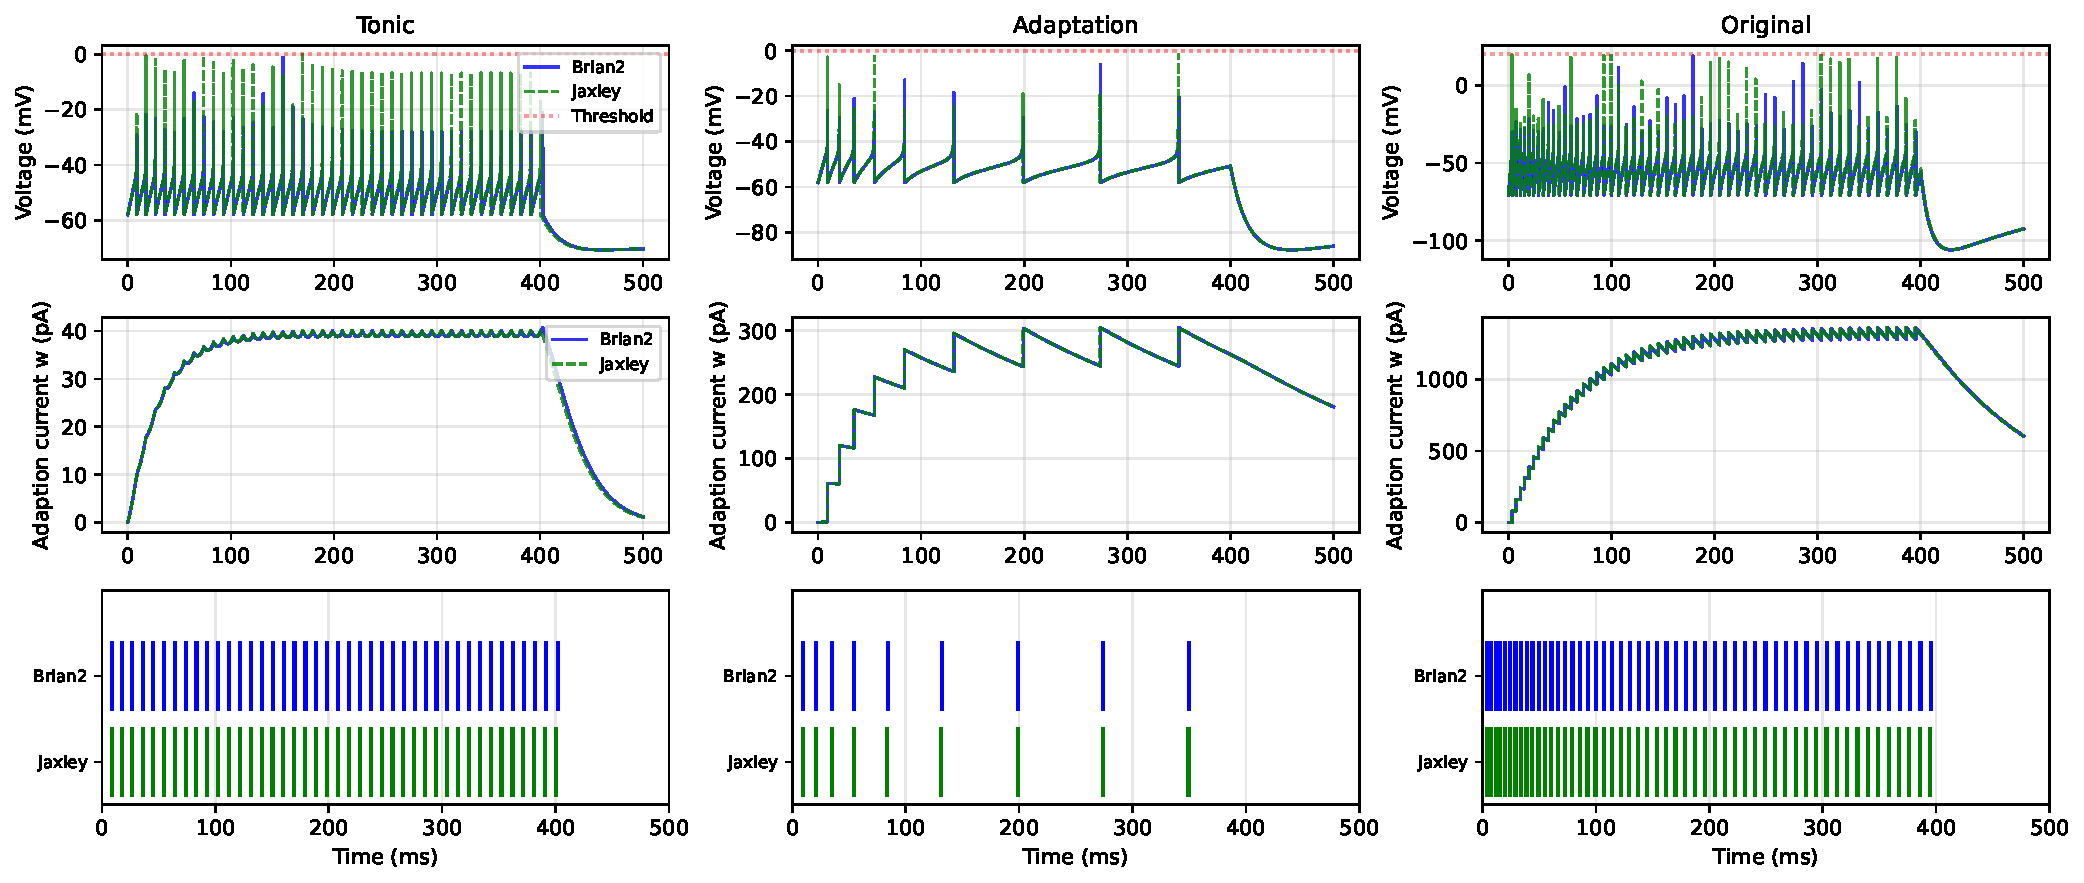
\includegraphics[width=\textwidth]{figures/adex_comparison_combined.pdf}
  \end{center}
  \caption{Comparison of our \texttt{Jaxley} \gls{AdEx} implementation against Brian2 across three reference parameter sets.
Left to right: tonic, adaptation and original parameters.
Tonic and adaptation parameters refer to the parameters provided by \cite{Naud2008}, original parameters are the parameters used in the original AdEx paper \cite{Brette2005}.
Top row shows the simulated voltage traces;
note that when the threshold is reached, the voltage is reset within the same time step --- a behaviour that becomes important when thinking about loss functions later on.
Second row displays the adaptation current $w$.
Last row compares the spike timings between \texttt{Brian2} and \texttt{Jaxley}.}\label{fig:brian_comparison}
\end{figure*}

This validation matters for two reasons.
First, it establishes that an \gls{AdEx}-style simplified neuron --- with its discrete reset and exponential spike initiation --- can be expressed cleanly inside a framework otherwise designed for \gls{HH}-type compartmental models.
The same implementation pattern carries over to other simplified models such as \gls{LIF} and Izhikevich, so the contribution is not strictly limited to \gls{AdEx}.
Second, and more importantly for the rest of this chapter: every optimisation failure we report from here on can be discussed as a property of gradient-based training and loss-function design, rather than as a possible artefact of the underlying dynamics.
The forward model is not the bottleneck.

\subsection{Surrogate Channel Verification}\label{sec:results:verification:surrogate}
\begin{figure*}
  \begin{center}
    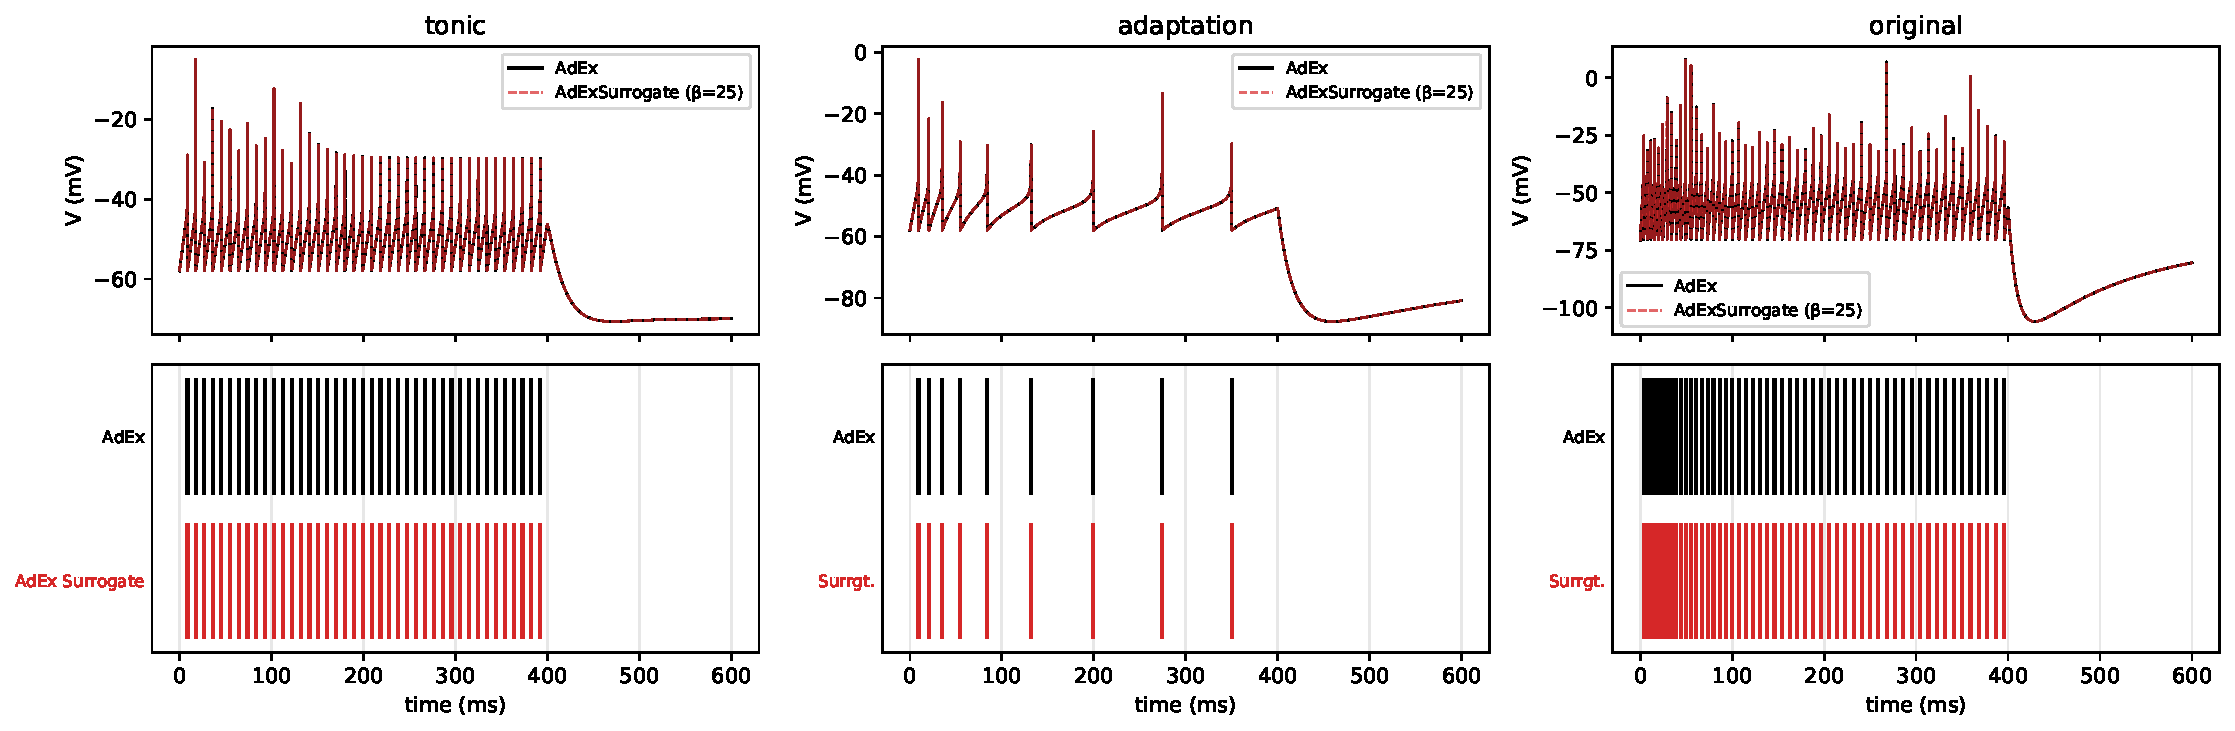
\includegraphics[width=\textwidth]{figures/surrogate_vs_non-surrogate_comparison}
  \end{center}
  \caption{Comparison of \texttt{AdEx} and \texttt{AdExSurrogate} channels. Both produce identical voltage traces as expected.}\label{fig:surrogate-channel-verification}
\end{figure*}

We run the two-part verification protocol of \cref{sec:method:surrogate-gradients:verification}.
On all three Naud parameter sets, the forward pass of \texttt{AdExSurrogate} matches the standard \texttt{AdEx} channel perfectly.
Both voltage trace and spike times are identical as can be seen in \cref{fig:surrogate-channel-verification}.
For the gradient-existence check, both channels report $\mathcal{L} = -21$ on the tonic set at the operating point; the gradients are summarised in \cref{tab:surrogate-gradient}.

\begin{table}[h]
  \centering
  \caption{Gradient of the negative spike count with respect to \texttt{v\_threshold} on the tonic parameter set ($\mathcal{L} = -21$ in all rows).}\label{tab:surrogate-gradient}
  \begin{tabular}{lr}
    \toprule
    Channel & $\partial\mathcal{L}/\partial v_{\text{th}}$ \\
    \midrule
    \texttt{AdEx} (hard threshold)                       & $0$ exactly \\
    \texttt{AdExSurrogate}, sigmoid ($\beta = 10$)       & $+1.9 \times 10^{-21}$ \\
    \texttt{AdExSurrogate}, exponential ($\beta = 5$)    & $+4.5 \times 10^{-4}$ \\
    \texttt{AdExSurrogate}, SuperSpike ($\beta = 10$)    & $+1.3 \times 10^{-1}$ \\
    \bottomrule
  \end{tabular}
\end{table}

The hard channel returns a structural zero; all three surrogates return a finite gradient of the correct sign.
At a fixed operating point the magnitudes span more than twenty orders of magnitude --- a property of the surrogate family alone (cf.\ \cref{fig:surr_grads}) --- which couples directly to learning-rate sensitivity in \cref{sec:results:training}.

%%%%%%%%%%%%%%%%%%%%%%%%%%%%%%%%%%%%%%%%%%%%%%%%%%%%%%%%%%%%%%%%%%%%%%%%%%%%
\section{Loss Function Analysis}\label{sec:results:landscape}

Before we report parameter-recovery numbers in \cref{sec:results:training}, this section characterises the geometry of the loss surfaces.
The motivation is diagnostic: a flat success/failure number does not say \emph{why} the method fails.
The recovery-radius benchmark in \cref{sec:results:baseline} will show that all three differentiable losses fail --- they do so for different reasons.
We therefore look at the shape of each loss directly: the position of the spiking valley, the extent of the non-spiking plateau, and the direction of the gradient on that plateau.
The geometric features predict the failure modes the benchmark later confirms.

For every $\binom{8}{2}=28$ pair of trainable parameters we evaluate four differentiable losses (\gls{MSE}, \gls{SDTW}, the Guarino feature-based loss, and the Van Rossum distance) on a $20\times 20$ grid spanning the parameter bounds;
the remaining six parameters are held at the Naud \texttt{adaptation} reference values of \cref{sec:method:adex:verification}.
The same grid evaluation produces a paired gradient field $\nabla_{\theta}\mathcal{L}$ via JAX autodiff.
Gradient computations were performed using a sigmoid surrogate with $\beta = 5.0$.
The magnitude is displayed for the 5 parameters used in the benchmark (for compute time reasons).
Loss and gradient panels can be found in \cref{sec:app:loss};

\subsection{Shared structure across losses}\label{sec:results:landscape:shared}
Three features recur across every loss surface we plot (\cref{sec:app:loss}):
\begin{itemize}
  \item \textbf{Narrow low-loss valleys.} The spiking region forms thin, curved valleys rather than isotropic (round, bowl shaped) basins.
        Valleys are often parallel to one axis (e.g.\ $g_L$--$E_L$ trades off along a single direction),
        meaning small updates along the wrong axis leave the loss unchanged.
  \item \textbf{Large non-spiking plateaus.} Substantial regions of parameter space yield a constant (or near-constant) loss because no spikes are produced and the loss reduces to a target-only constant.
        Soft spike-detection terms supply a residual gradient on these plateaus, but the gradient is small and its direction is not constrained by the true distance to the spiking valley.
  \item \textbf{Plateau gradient magnitude, not direction.} On the spike-aware losses (Guarino, Van Rossum) the surrogate can supply a small but non-zero gradient on the non-spiking plateau via $\sigma'(V - V_{\mathrm{th}})$.
        The resulting gradient direction does not point necessarily toward the spiking transition, see \cref{fig:guarino-landscape-focus}.
        In any case, its magnitude is several orders below the gradient inside the spiking region.
\end{itemize}

The three subsections that follow show what these shared features look like in each loss individually.
Before that a word about how gradient magnitudes vary between parameters.

\subsubsection*{Gradient magnitude asymmetry between parameters}

\begin{figure}[t]
  \begin{center}
    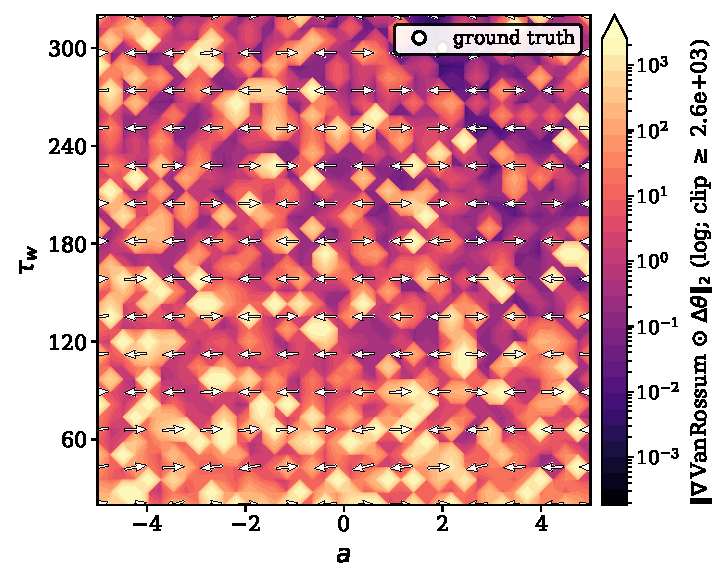
\includegraphics[width=0.7\textwidth]{figures/loss_landscape_focus_vanrossum_a_tau_w_grad2d_superspike_10.pdf}
  \end{center}
  \caption{Van Rossum bound-normalised gradient field on the $a$--$\tau_w$ plane in the \texttt{adaptation} scenario (ground truth $a=2$\,nS, $\tau_w=300$\,ms).
SuperSpike surrogate, $\beta=10$.
The colour scale spans six orders of magnitude in bound-normalised sensitivity, but the quiver is dominated by the horizontal component throughout: $|\partial\mathcal{L}/\partial a \cdot \Delta a| \gg |\partial\mathcal{L}/\partial \tau_w \cdot \Delta \tau_w|$ across the whole slice.}\label{fig:vanrossum-a-tauw}
\end{figure}

There are huge differences between how susceptible to change different parameters are.
\Cref{fig:vanrossum-a-tauw} shows the bound-normalised gradient field on the $(a, \tau_w)$ plane around the Naud \texttt{adaptation} reference point ($a=2$\,nS, $\tau_w=300$\,ms), under Van Rossum with SuperSpike $\beta=10$.
The quiver is dominated by the horizontal ($a$) component at essentially every grid cell, even after bound-normalisation puts the two axes on the same dimensionless scale.
This is a real geometric property, not the unit-scaling artefact.
It is mostly explained by a structural asymmetry in how AdEx parameters enter the dynamics.
One class ($E_L$, $g_L$, $C_m$, $V_T$, $a$) enters the right-hand side of the membrane or adaptation equation at every timestep, so a small perturbation rescales or shifts $V(t)$ (or $w(t)$) at every point along the trajectory and accumulates loss sensitivity over the full integration window.
A second class ($b$, $\tau_w$, $\Delta_T$) only feeds into the dynamics through narrow channels.
$b$ acts as a discrete kick on $w$ at spike times, so its gradient is gated by spike events and vanishes whenever the cell is silent or near-silent.
$\tau_w$ is a relaxation timescale whose effect is only visible in longer simulations.
$\Delta_T$ enters an exponential whose value is dominated by $V_T$ at most operating points.
The bound-normalised gradient field inherits this asymmetry directly.
Rescaled units cannot make $b$ act outside spike events, nor make $\tau_w$ act on timescales the stim window does not visit.
The $(a, \tau_w)$ slice above is one instance of this pattern; the same imbalance recurs whenever a continuously-acting parameter is paired with an event-driven or timescale one, and it is one of the reasons $b$ and $\tau_w$ are systematically harder to recover.

\subsection{Mean Squared Error: the non-spiking attractor}\label{sec:results:landscape:mse}

\begin{figure}[t]
  \begin{center}
    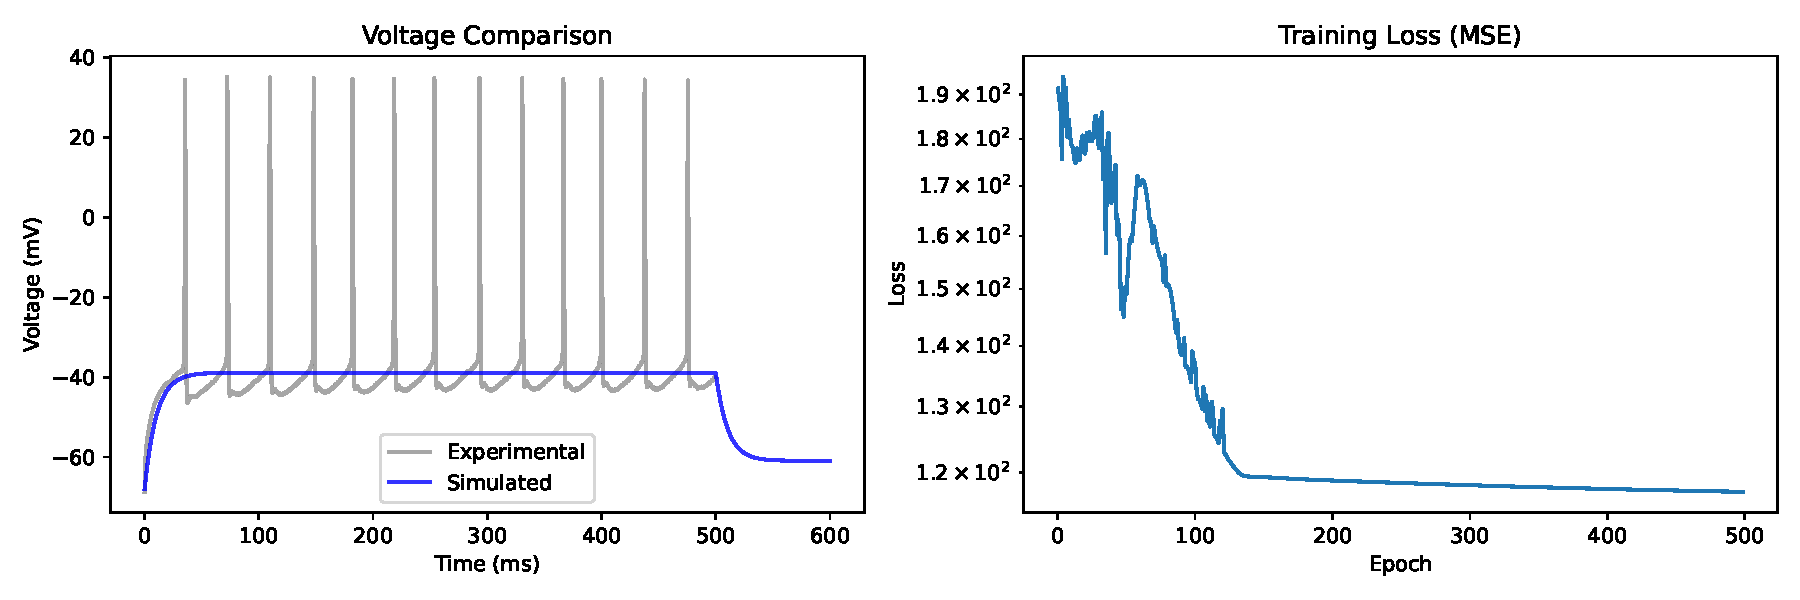
\includegraphics[width=0.95\textwidth]{figures/mse_training_results.pdf}
  \end{center}
  \caption{
\gls{MSE} training result on voltage recordings of a mouse straital projection neuron.
(a) The optimiser converges to a non-spiking subthreshold solution (blue) that tracks the experimental resting potential but produces no spikes.
(b) The loss decreases monotonically, confirming that the non-spiking solution is a genuine local minimum of the \gls{MSE} objective --- eliminating spikes reduces point-wise error more effectively than aligning them.
}\label{fig:mse-training-results}
\end{figure}

The \gls{MSE} surface has visibly the most amount of local minima.
This reflects the behaviour that for different spike counts, the loss function performs best in the most similar subthreshold regimes.
Across all 28 parameter pairs the surfaces display thin, axis-aligned spiking valleys.
We observe large magnitudes in parameter areas where VanRossum and Guarino show small loss values.
This indicates that error is aggregated based on small timing mis-alignments.

This geometry has an immediate empirical signature in training: starting from a tonic spiking initialisation, the \gls{MSE} optimiser deletes the simulated spikes rather than aligning them, because deleting spikes is the easier to reach loss target.
\Cref{fig:mse-training-results} shows the resulting trajectory on voltage recordings of a mouse straital projection neuron:
the trace tracks the resting potential with no spikes, and the loss decreases monotonically across all $50$ epochs.
\gls{MSE}'s plateau gradient therefore points \emph{away} from the spiking valley rather than toward it.

\subsection{Guarino: feature artifacts everywhere}\label{sec:results:landscape:guarino}

The Guarino feature-based loss replaces \gls{MSE}'s point-wise voltage comparison with a weighted sum of relative errors on eight discrete spike features (\cref{sec:method:opt:loss:feature-loss}).
This can be supplemented by a soft validity penalty whenever the simulated trace does not produce enough spikes to evaluate a feature.
Both changes target the failure mode diagnosed for \gls{MSE}: removing spikes is no longer cheaper than aligning them, because the missing-feature penalty contributes a fixed positive term to the loss whenever a feature cannot be evaluated.
The geometry near a spiking ground truth reflects this redesign.

\Cref{fig:guarino-landscape-focus} shows the loss and the gradient field on the $E_L$--$g_L$ plane around the Naud \texttt{adaptation} reference point, on a logarithmic scale that spans six orders of magnitude.
A narrow curved valley (dark purple, $\mathcal{L} \lesssim 10^{0}$) contains the ground truth and traces the locus where the leak equilibrium and conductance jointly produce the correct spike count and timing.
In the top left corner, the missing-feature penalty turns on as the simulated trace loses spikes;
The plateau is bounded on the upper-left by a sharp yellow ridge ($\mathcal{L}\sim 10^{5}$).
This is an interesting artifact of the feature based loss we constructed: the non-spiking area attributes a fixed penalty per feature.
Paramaters within the yellow ridge area produce voltage traces with a single or very little spikes.
This disables the fixed added penalty, and instead large errors (e.g. in spike frequency) lead to huge loss values --- gradient signals on the plateau therefor \emph{discourage} from moving into the optimal direction.
All of this behaviour is basically irrelevant for sampling-based losses, which indicates why Guarino performs well in the benchmark when combined with Nelder-Mead.

\begin{figure}[t]
  \begin{center}
    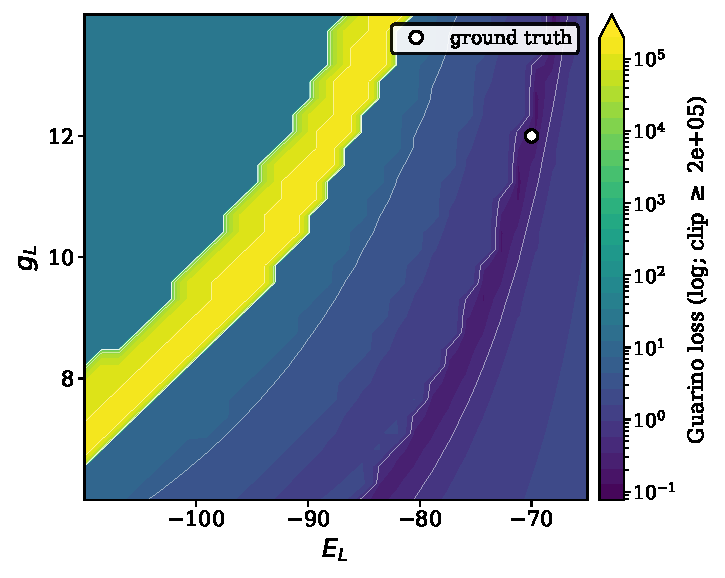
\includegraphics[width=0.49\textwidth]{figures/guarino_focus_E_L_g_L_loss.pdf}\hfill
    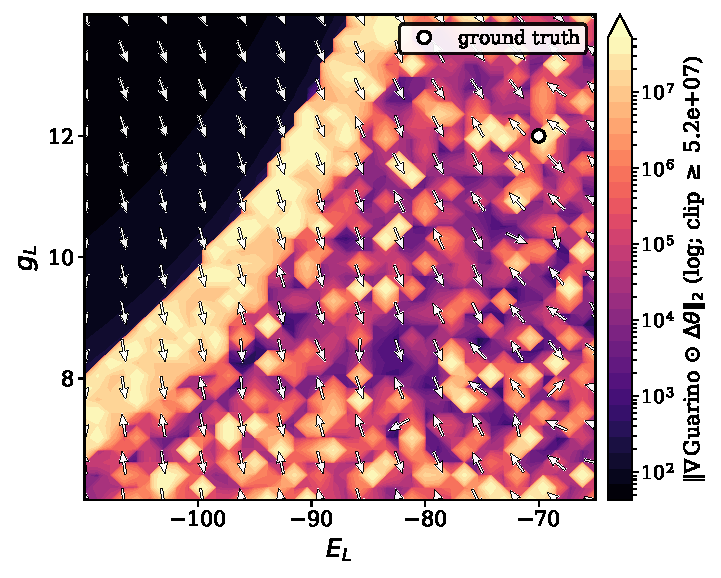
\includegraphics[width=0.49\textwidth]{figures/guarino_focus_E_L_g_L_grad.pdf}
    %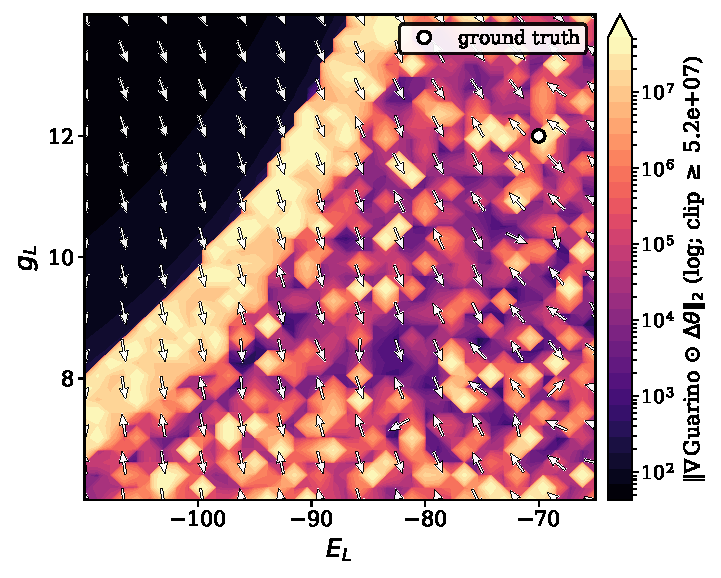
\includegraphics[width=0.49\textwidth]{figures/loss_landscape_focus_guarino_E_L_g_L_grad2d_superspike_10.pdf}
  \end{center}
  \caption{Guarino loss landscape (left) and bound-normalised gradient field (right) on the $E_L$--$g_L$ plane around the Naud \texttt{adaptation} reference point.
SuperSpike surrogate, $\beta = 10$.
Left: $\mathcal{L}_{\mathrm{Guarino}}$ on a log scale spanning six orders of magnitude.
Right: $\|\nabla\mathcal{L}\odot\Delta\theta\|_{2}$ on a log scale.
Arrows show the unit direction of steepest \emph{ascent} in bound-normalised coordinates; the optimiser steps opposite.
The ground-truth marker sits inside the narrow curved valley of low loss (dark purple, left), bounded on the upper-left by the low spike frequency, high loss penalty ridge (yellow),
The top left corner shows the plateau where the simulated trace loses all spikes.
On the right panel the penalty ridge dominates the gradient magnitude ($\sim 10^{7}$).
The plateau gradient outside the ridge is non-zero ($\sim 10^{2}$--$10^{3}$ in bound-normalised units) and uniformly directional, pointing south-east toward the ridge.}\label{fig:guarino-landscape-focus}
\end{figure}

Overall we can make three observations the right panel of \cref{fig:guarino-landscape-focus}.
First, $\|\nabla\mathcal{L}\odot\Delta\theta\|_{2}$ spans five orders of magnitude across this single slice: $\sim 10^{2}$ in the plateau interior to $\sim 10^{7}$ on the penalty ridge.
Second, on the non-spiking plateau the gradient field is approximately uniform --- arrows point in essentially the same south-east direction across a region tens of millivolts wide, and that direction is the descent direction toward the ridge, whereas on the other side of the ridge, gradient behaviour is a lot more chaotic, varying over multiple orders of magnitude between evaluated points.
Third, the largest gradients sit on the penalty ridge itself, not at the ground truth.
All of this highlight the difficulties when applying feature based losses to gradient methods.
The sheer amount of hyperparameter needed to successfully finetune this loss may simply be too high (features specific weights, penalties, smoothness parameters, ...).

\subsection{Van Rossum: a smoother loss, still chaotic gradient}\label{sec:results:landscape:vanrossum}

The Van Rossum distance (\cref{sec:method:opt:loss:van-rossum}) is the only loss in our comparison that supplies a smooth path from the spike train $s(t)$ to the loss value: the exponential kernel $K$ and the $L^{2}$ norm are themselves differentiable, so no softness hyperparameter is required to make the loss path smooth.
The geometric prediction is that the Van Rossum surface should be smoother in the spiking regime than Guarino's --- the kernel convolution averages over a $\tau_{\mathrm{kernel}}$-wide window, so small spike-timing perturbations no longer produce discrete penalty-ridge transitions.
The empirical picture in the bound-normalised gradient field is more nuanced.

\Cref{fig:vanrossum-grad-focus} shows the Van Rossum loss and gradient field on the same $E_L$--$g_L$ slice and surrogate configuration as the Guarino panel of \cref{fig:guarino-landscape-focus} (SuperSpike, $\beta=10$), so the two figures differ only in the loss.

\begin{figure}[t]
  \begin{center}
    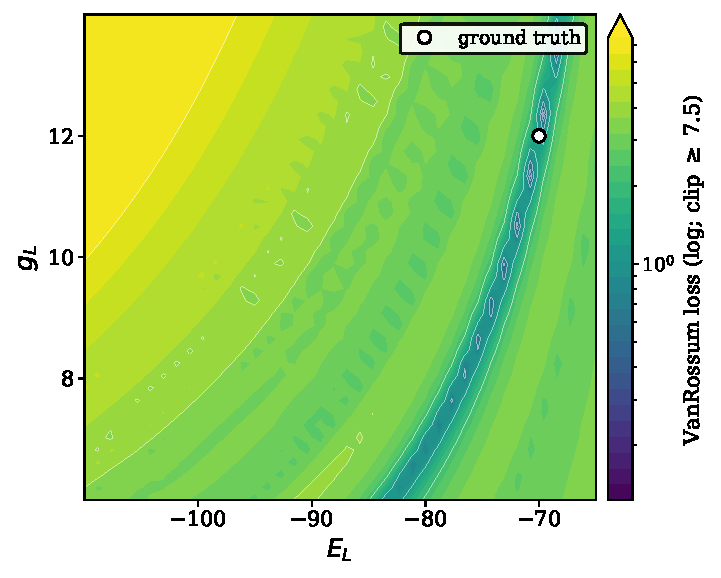
\includegraphics[width=0.49\textwidth]{figures/vanrossum_focus_E_L_g_L_loss.pdf}\hfill
    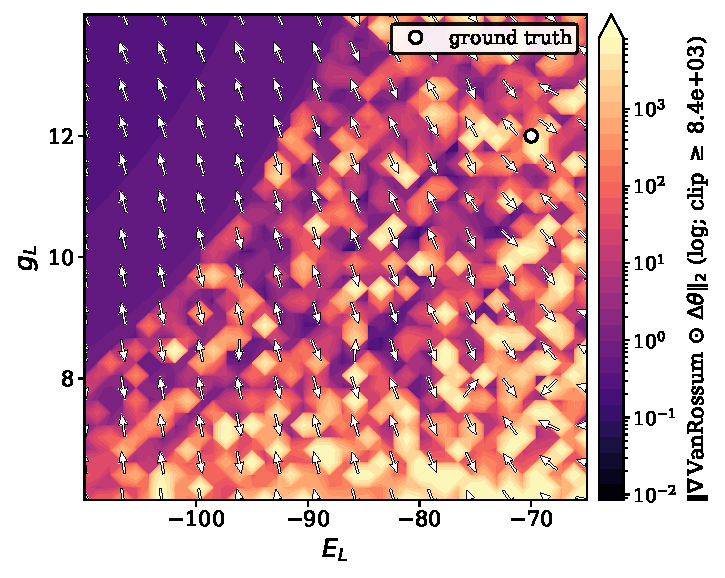
\includegraphics[width=0.49\textwidth]{figures/vanrossum_focus_E_L_g_L_grad.pdf}
  \end{center}
  \caption{$E_L$--$g_L$ plane around the Naud \texttt{adaptation} reference point. Left: Van Rossum loss, RightL: bound-normalised gradient-norm landscape with quiver overlay.
SuperSpike surrogate, $\beta=10$, matched to \cref{fig:guarino-landscape-focus}.
Left: $\mathcal{L}_{VR}$ on a log scale spanning below two orders of magnitude.
Right: $\|\nabla\mathcal{L}\odot\Delta\theta\|_{2}$ on a log scale.
Arrows show the unit direction of steepest \emph{ascent} in bound-normalised coordinates; the optimiser steps opposite.
The upper-left non-spiking plateau carries a small ($\sim 10^{-1}$) but directionally consistent ascent gradient.
The lower-right spiking region exhibits a granular pattern of order-of-magnitude jumps between neighbouring grid cells:
the surrogate's narrow active window plus the binary $s(t)$ mean that a single grid step can shift a spike in or out of the trace, producing a discrete change in $K \ast s(t)$ and a step change in $\|\nabla\mathcal{L}\|$.}\label{fig:vanrossum-grad-focus}
\end{figure}

Two contrasts with the Guarino panel stand out.
First, the feature penalty ridge of \cref{fig:guarino-landscape-focus} is absent:
Van Rossum has no discrete penalty for losing a 'feature', so the loss climbs monotone and smoothly from valley to plateau across the diagonal transition rather than jumping by four orders of magnitude.
This is aided by the kernel-smoothing effect the design argument predicts (\cref{sec:method:opt:loss:van-rossum}).
Second, the bound-normalised plateau gradient is much smaller for Van Rossum ($\sim 10^{-1}$) than for Guarino ($\sim 10^{2}$):
without the validity-flag penalty's soft-gated contribution, the only signal on the plateau comes from $\sigma'(V - V_{\mathrm{th}})$ in the brief window when the leak dynamics carry $V$ near threshold, which on the non-spiking plateau happens rarely or not at all.
The kernel-smoothing benefit on the spiking branch is therefore paid for by a weaker plateau gradient on the non-spiking branch.
This could be described as a magnitude bottleneck, and explains the non-moving parameters in non spiking starting configuations.

The spiking region (lower-right of the diagonal) is \emph{not} the smooth basin the kernel-convolution argument would suggest in isolation.
Instead, it is dominated by a high-contrast checkerboard of bright and dark patches whose magnitudes differ by an order of magnitude between neighbouring grid cells.
This might be explained by the binary indicator $s(t)$: small parameter perturbation can shift one spike's threshold-crossing across a single timestep and add or remove an event from the trace.
The Van Rossum loss reads this as a discrete jump in $K \ast s(t)$, and the autodiff backward pass attributes the jump via \texttt{custom\_vjp} to the surrogate kernel at that timestep, producing a gradient at the affected grid cell that is large but uncorrelated with its neighbours' gradients.
The kernel convolution smooths the loss over timing perturbations of \emph{existing} spikes;
it does not smooth over spike-count changes, which is what dominates the region near and beyond the ground truth at any finite $\beta$.

\subsubsection*{Surrogate-family dependence}

\Cref{fig:vanrossum-surrogate-sweep} reports the same Van Rossum gradient field on the same slice for SuperSpike and sigmoid surrogates at three slopes $\beta\in\{5,10,25\}$.
All six panels use identical axes, the same loss, and the same forward simulation; only the backward-pass surrogate kernel changes.

\begin{figure}[t]
  \begin{center}
    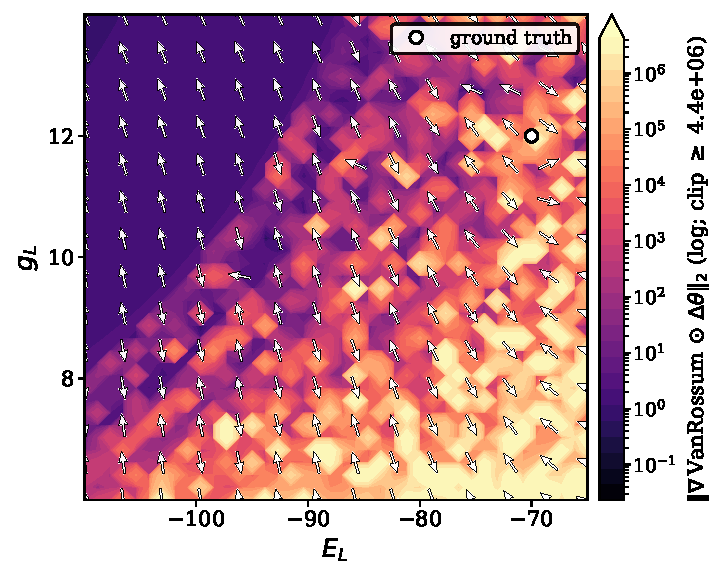
\includegraphics[width=0.32\textwidth]{figures/loss_landscape_focus_vanrossum_E_L_g_L_grad2d_superspike_5.pdf}\hfill
    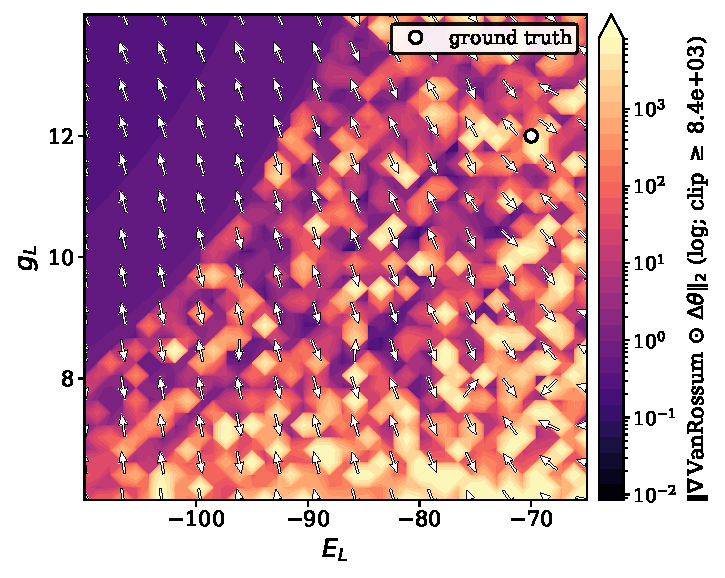
\includegraphics[width=0.32\textwidth]{figures/loss_landscape_focus_vanrossum_E_L_g_L_grad2d_superspike_10.pdf}\hfill
    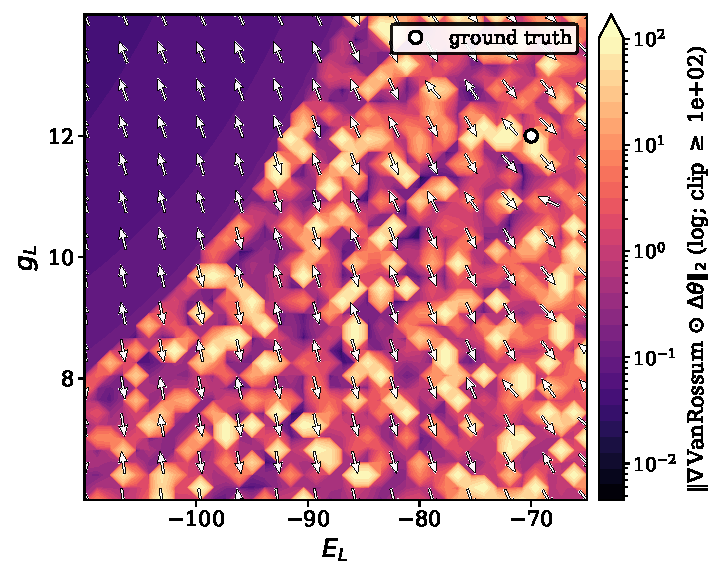
\includegraphics[width=0.32\textwidth]{figures/loss_landscape_focus_vanrossum_E_L_g_L_grad2d_superspike_25.pdf}\\[0.5em]
    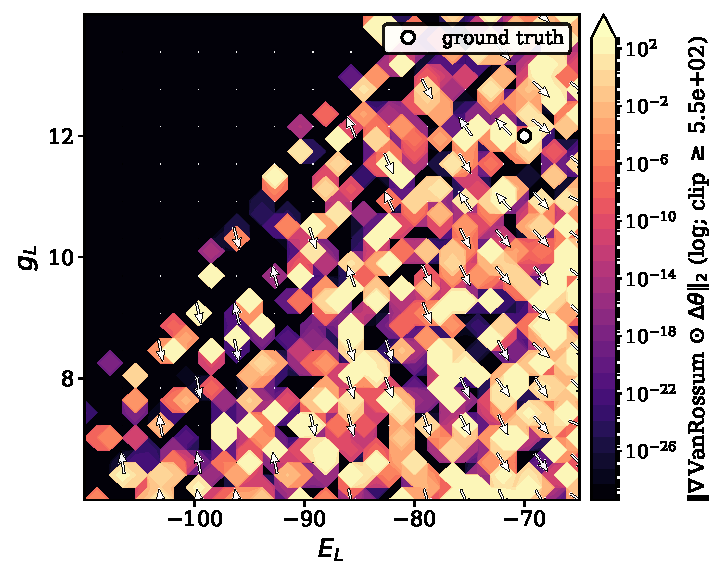
\includegraphics[width=0.32\textwidth]{figures/loss_landscape_focus_vanrossum_E_L_g_L_grad2d_sigmoid_5.pdf}\hfill
    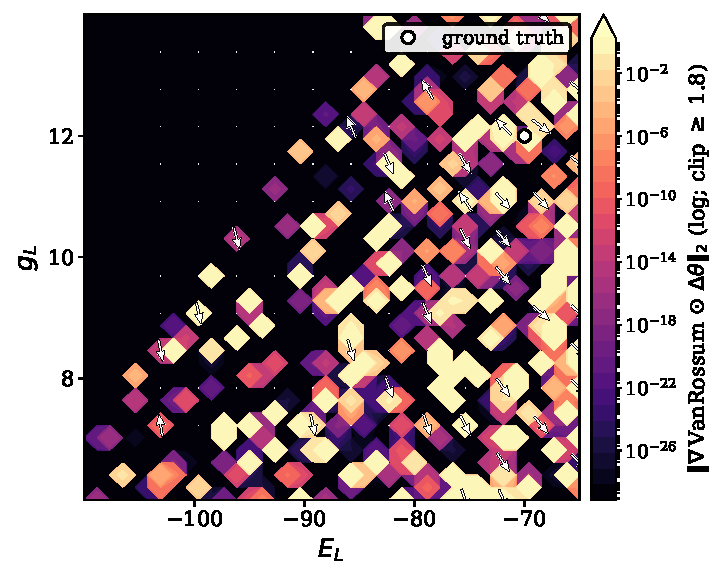
\includegraphics[width=0.32\textwidth]{figures/loss_landscape_focus_vanrossum_E_L_g_L_grad2d_sigmoid_10.pdf}\hfill
    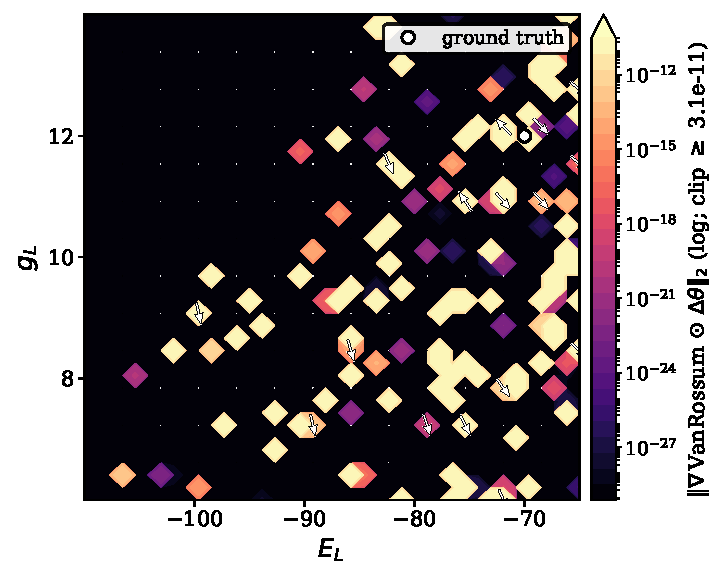
\includegraphics[width=0.32\textwidth]{figures/loss_landscape_focus_vanrossum_E_L_g_L_grad2d_sigmoid_25.pdf}
  \end{center}
  \caption{Van Rossum bound-normalised gradient field on the $E_L$--$g_L$ plane around the Naud \texttt{adaptation} reference point, swept over surrogate family and slope.
Top row: SuperSpike ($\beta=5, 10, 25$). Bottom row: sigmoid ($\beta=5, 10, 25$).
SuperSpike's heavy tail $1/(\beta|x|+1)^2$ produces gradient signal across the entire plane at every $\beta$: spiking-region magnitudes shrink from $\sim 10^{6}$ at $\beta=5$ to $\sim 10^{2}$ at $\beta=25$, but the spatial coverage is preserved.
The sigmoid's exponentially-suppressed $\sigma'(\beta x) = \sigma(\beta x)(1-\sigma(\beta x))$ collapses to numerical noise off-threshold: the dead zone (black) covers the non-spiking plateau at $\beta=5$, most of the slice at $\beta=10$, and the entire plane at $\beta=25$ (magnitudes reach $10^{-27}$, well below denormalised float32 precision).}\label{fig:vanrossum-surrogate-sweep}
\end{figure}


%%%%%%%%%%%%%%%%%%%%%%%%%%%%%%%%%%%%%%%%%%%%%%%%%%%%%%%%%%%%%%%%%%%%%%%%%%%%
\section{Parameter Recovery}\label{sec:results:training}

We now turn from the geometry of the loss surfaces to what happens when an optimiser actually descends them.
Throughout this section we follow the benchmark setup from \cref{sec:method:opt:recovery-benchmark}.
The section is organised in two parts.
\Cref{sec:results:positive-example} presents a single worked example in which gradient-based recovery succeeds somewhat;
enough to establish that the approach is viable in principle, but already revealing that the problem is under-constrained.
%\Cref{sec:results:real-singletrace} presents an attempt on fitting parameters to real voltage recordings.
\Cref{sec:results:baseline} then reports the recovery-radius benchmark: three differentiable losses against two Nelder--Mead baselines on matched initialisations.
The benchmark is the headline result of the chapter, and the picture it produces is uncomfortable:
on every scenario and every perturbation scale, gradient-based recovery performs similar or below the no-optimisation baseline.
Nelder--Mead on the same objective recovers reliably better.
The geometric features of \cref{sec:results:landscape} suggest this pattern in advance.

\subsection{A Worked Example: Recovering a Tonic AdEx Cell}\label{sec:results:positive-example}
Before turning to the per-loss breakdown and the systematic benchmark, we present one configuration in which gradient-based fitting succeeds cleanly.
The ground truth is the Naud tonic parameter set (\cref{sec:method:adex:verification}); the six trainable membrane parameters $\{C_m, g_L, V_r, V_T, E_L, \Delta_T\}$ are perturbed by approximately $15\,\%$ of their bound range, and the optimiser is run for $50$ epochs of single-stage training under the Guarino feature-based loss (\cref{sec:method:opt:loss:feature-loss}).
The adaptation parameters $\{a, b, \tau_w\}$ are held at ground truth, matching the scope fixed for the recovery-radius benchmark in \cref{sec:method:opt:recovery-benchmark:scope}.
\Cref{fig:guarino-synthetic-recovery} reports the outcome.

\begin{figure}[t]
  \begin{center}
    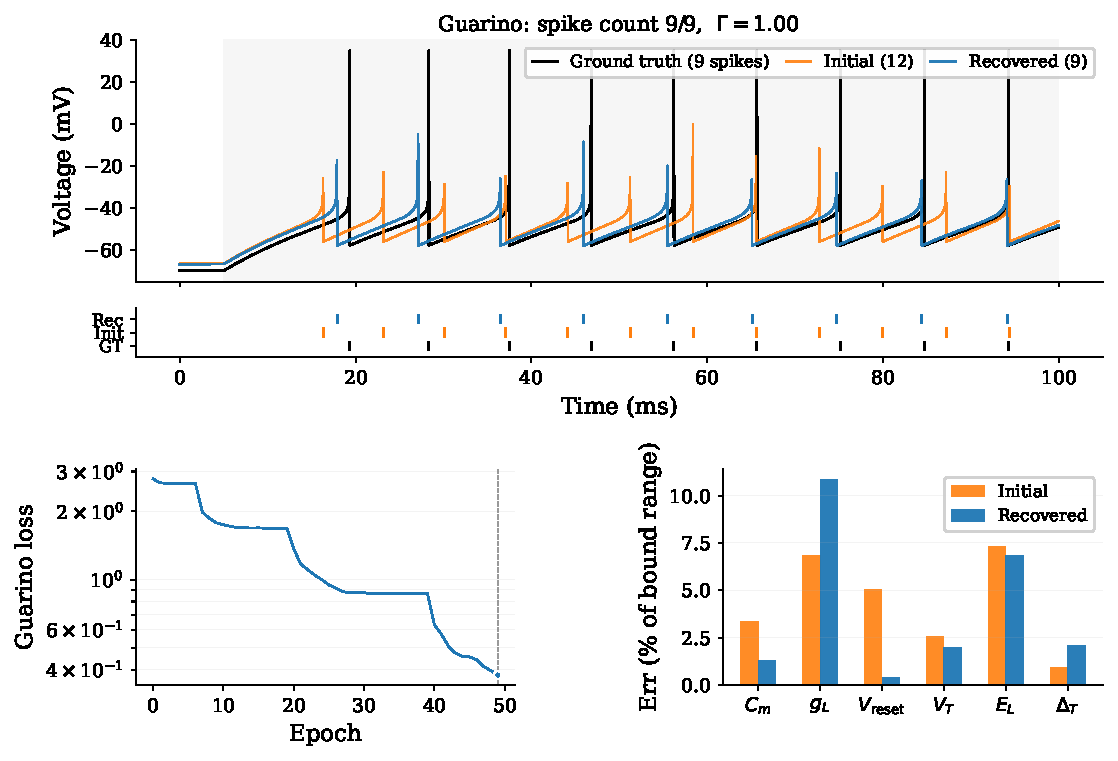
\includegraphics[width=\textwidth]{figures/guarino_synthetic_recovery}
  \end{center}
  \caption{Single-stage recovery of a tonic \gls{AdEx} cell under the Guarino loss.
Top: voltage traces of the ground truth (black, $9$ spikes), the perturbed initialisation (orange, $7$ spikes) and the recovered fit (blue, $9$ spikes), with the corresponding spike raster below.
Bottom left: training loss across $50$ epochs; the dashed line marks the epoch at which the best parameters were retained.
Bottom right: per-parameter absolute error before and after training, normalised by the width of the parameter bounds.}\label{fig:guarino-synthetic-recovery}
\end{figure}

At the trace level the recovery is visually convincing.
The perturbed initialisation produces $12$ spikes against the target's $9$ and misses most spike times by several milliseconds; after training the recovered trace matches the ground truth spike-for-spike and yields a coincidence factor of $\Gamma = 1.00$ at the $\Delta = 2\,\text{ms}$ tolerance fixed in \cref{sec:method:opt:evaluation-metrics}.
The loss curve descends monotonically over roughly one order of magnitude, with the steepest drop concentrated between epochs $35$ and $45$ where the optimiser successfully finds the right spike count.

The per-parameter panel tells a more nuanced story.
Two of the six trainable parameters --- $C_m$ and $V_{\text{reset}}$ --- tighten substantially towards their ground-truth values.
However, other parameters change marginally or drift further away from the ground truth.
Especially $g_L$'s final error greatly exceeds the initial perturbation.
The optimiser is therefore not recovering the parameter vector pointwise;
it is settling into a local minima combination that reproduces the target spike train while trading error across correlated axes.
The loss-landscape evidence behind this compensation is taken up in \cref{sec:results:landscape}, and its implications for parameter identifiability are discussed in \cref{ch:discussion}.

This success is not generic.
The same loss, the same hyperparameters and the same ground-truth parameter set fail to recover a comparable fit once the perturbation is increased, the firing regime is changed, or the adaptation parameters are made trainable.
The recovery-radius benchmark of \cref{sec:results:baseline} quantifies how quickly the success region closes;
the geometric counterpart in \cref{sec:results:landscape} explains why.

%%%%%%%%%%%%%%%%%%%%%%%%%%%%%%%%%%%%%%%%%%%%%%%%%%%%%%%%%%%%%%%%%%%%%%%%%%%%

% \subsection{A worked example: fitting an IDthresh recording}\label{sec:results:real-singletrace}
%
% The second worked example fits a real cell.
% We use a voltage recording of a mouse's striatal projection neuron from the Johansson \& Silberberg striatal recordings~\cite{Johansson2020}, cleaned up and made usable by Kozlov et al. \cite{Kozlov2025}.
% The six trainable membrane parameters are the same as in \cref{sec:results:positive-example};
% the adaptation parameters $(a, b, \tau_w)$ are held at initial values (for tonic spiking).
%
% \begin{figure}[t]
%   \begin{center}
%     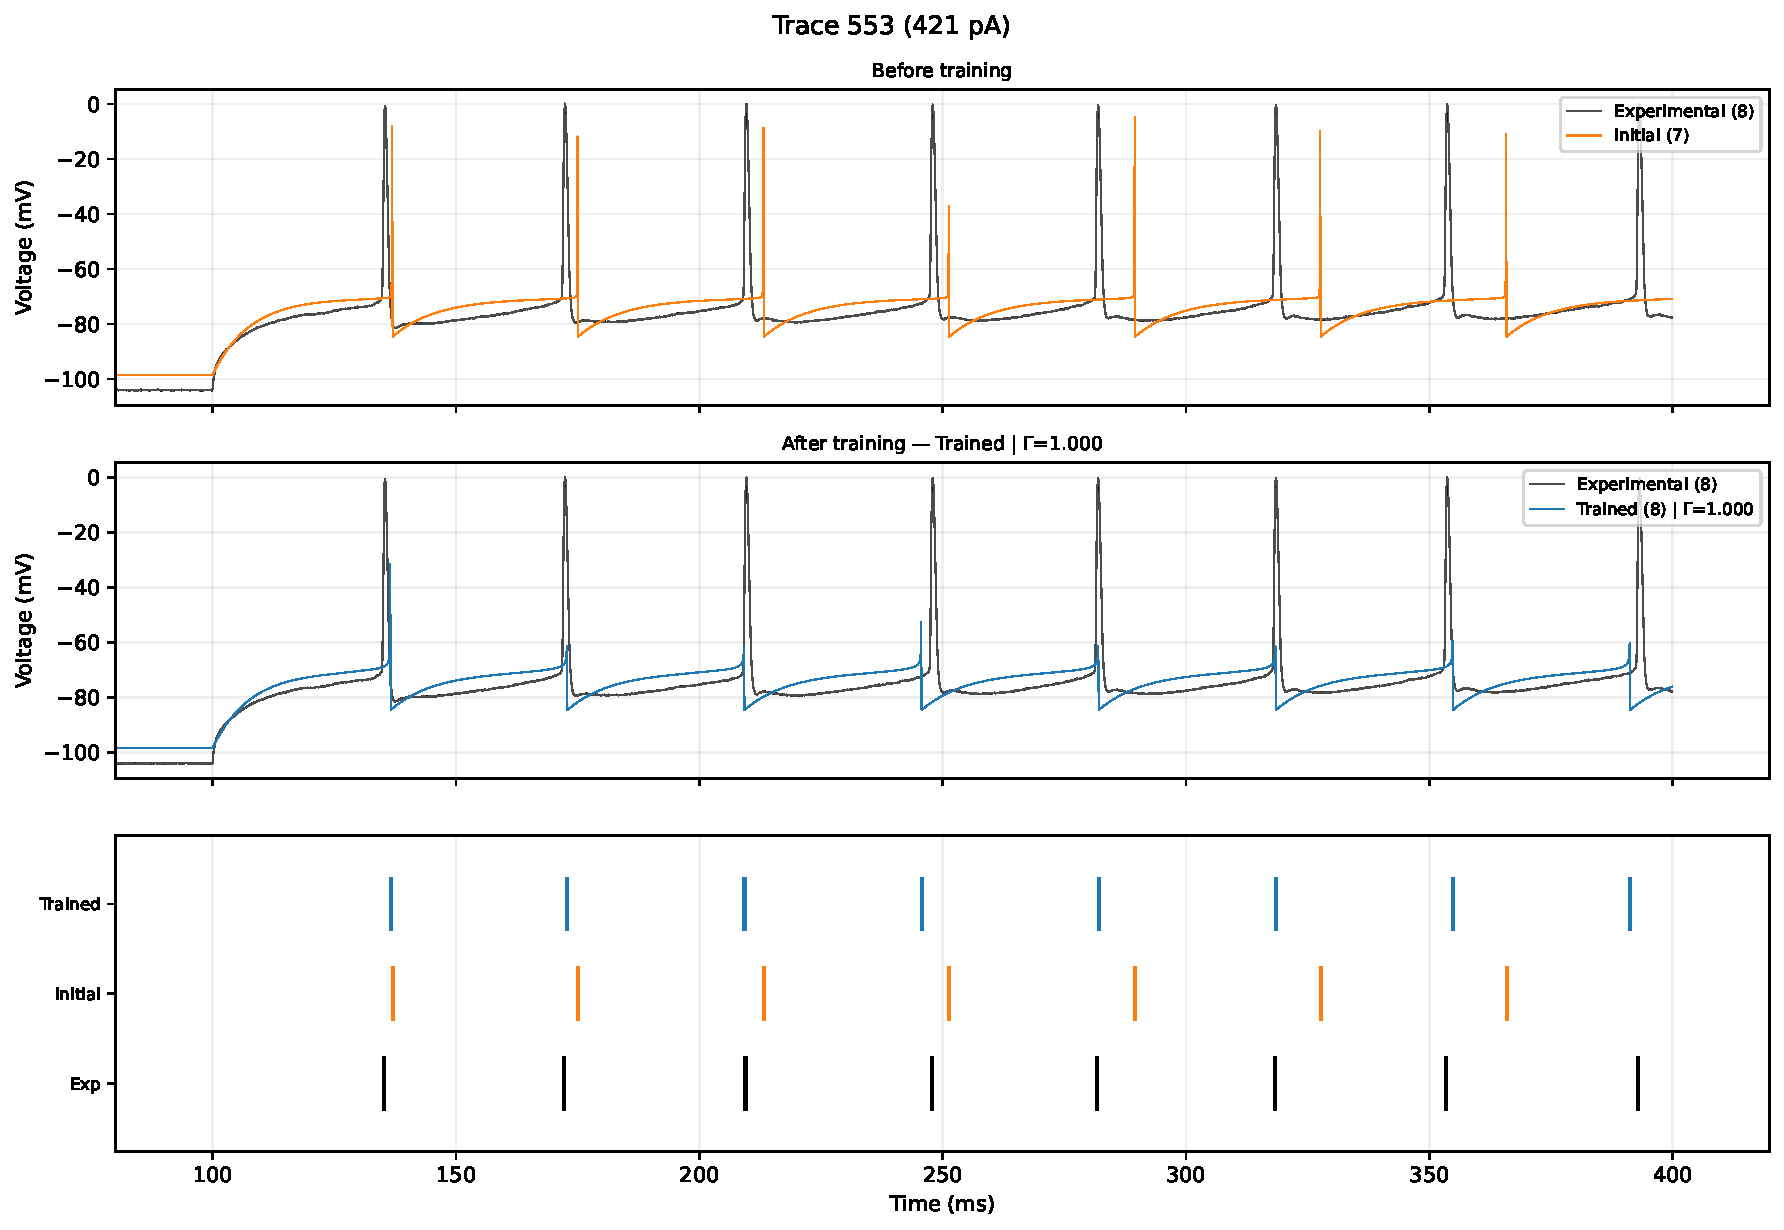
\includegraphics[width=\textwidth]{figures/real_singletrace_553_fit}
%   \end{center}
%   \caption{Gradient-based fit of an IDthresh recording ($I=421$\,pA, 8 target spikes).
% Top: voltage overlay before training (7 sim spikes, $\Gamma_{\mathrm{init}}=+0.411$).
% Middle: after $30$ Adam epochs (8 sim spikes, $\Gamma=+1.000$, all aligned within the $\Delta=2$\,ms coincidence window).
% Bottom: spike raster for experimental, initial and trained traces.}\label{fig:real-singletrace-fit}
% \end{figure}
%
% \Cref{fig:real-singletrace-fit} reports the outcome.
% The training loss falls from $3.28$ to $0.30$ over the first $30$ epochs;
% at the best-loss checkpoint (epoch $29$) the trained simulation produces $8$ spikes against the target's $8$, with $\Gamma=+1.000$ at $\Delta=4$\,ms tolerance.
% The largest parameter movement during training is $|\Delta C_m| \approx 0.17$\,pF on a bound range of $230$\,pF (one part in $1{,}300$); the other five parameters move by less.
% Subthreshold trajectories between spikes diverge visibly from the recording, but the spike count, firing frequency and all eight spike timings match within the coincidence-factor window.

\subsection{Recovery-Radius Benchmark}\label{sec:results:baseline}
The worked example of \cref{sec:results:positive-example} show that gradient-based recovery can be possible;
however, even a broken clock is right twice a day.
It does not establish how robust the recovery is, nor how it compares against a derivative-free baseline on the same objective.
The recovery-radius benchmark of \cref{sec:method:opt:recovery-benchmark} answers both questions on a single instrument: it aggregates parameter recovery over $5\,\text{methods}\times 3\,\text{scenarios}\times 6\,\text{perturbations}\times 30\,\text{directions}=2700$ paired runs, producing a recovery-success curve per method and a single recovery radius per (scenario, method) pair.

\subsubsection{Headline result: success vs.\ perturbation}
\Cref{fig:recovery-radius} shows $P(\Gamma > 0.5)$ as a function of the perturbation scale $\delta$, with one panel per scenario and one curve per method.
A no-optimisation floor (\texttt{init\_floor}, the success rate of the perturbed initialisation evaluated without any update) is included as a reference; methods below this floor have regressed.

\begin{figure*}[t]
  \begin{center}
    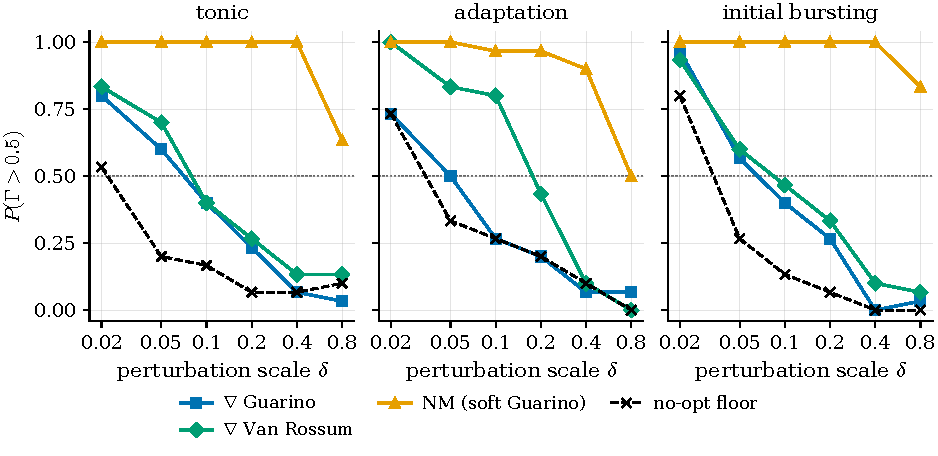
\includegraphics[width=\textwidth]{figures/recovery_radius_curves.pdf}
  \end{center}
  \caption{Recovery success $P(\Gamma > 0.5)$ as a function of the relative perturbation scale $\delta$, per scenario.
Each curve aggregates 30 paired random-direction perturbations; methods are evaluated on identical $(\theta^*+\delta u_k)$ initialisations within each scenario.
The $\Gamma > 0.5$ threshold follows \cref{sec:method:opt:evaluation-metrics}; the dashed horizontal at $0.5$ marks the success-probability level used to define the recovery radius.
\texttt{init\_floor} reports $\Gamma$ at the perturbed initialisation with no optimisation applied.}\label{fig:recovery-radius}
\end{figure*}

Four observations stand out.
First, all gradient methods perform similar or worse than the initialisation floor.
Even for tiny perturbations, the gradient approach struggled to faithfully recover original parameters.
Second, both Nelder--Mead variants dominate every gradient method on every scenario at every $\delta$: they have the largest recovery radii and the highest success rates inside them.
Third, \texttt{grad\_mse} performed consistently the worst, consistent with the \gls{MSE} landscape geometry of \cref{sec:results:landscape:mse}.
Fourth, the two Nelder--Mead variants are indistinguishable: \texttt{nm\_guarino} (soft features) and \texttt{nm\_guarino\_hard} (exact features) report identical $\delta_{50}\in\{0.2,0.2,0.4\}$ and identical median $\Gamma_{0.05}=+1.00$ on every scenario, with per-direction outcomes differing by at most one direction out of 30.\label{sec:results:nm-soft-vs-hard}

\subsubsection{Recovery radii}
\Cref{tab:results-summary} reports two summary statistics per (scenario, method) pair:
the recovery radius $\delta_{50}$ (the largest grid value of $\delta$ for which $P(\Gamma>0.5)\geq 0.5$) and the median $\Gamma$ over all directions at $\delta = 0.05$.
The median at $\delta = 0.05$ is the most diagnostic single number: $\delta = 0.02$ is too easy (every reasonable method scores well) and $\delta \geq 0.2$ is too hard for the gradient methods (most rows are non-spiking failures dominated by the surrogate's plateau gradient).

\begin{table}[t]
\centering
\caption{Recovery-radius benchmark summary. $\delta_{50}$ is the largest grid value of $\delta\in\{0.02,0.05,0.1,0.2,0.4,0.8\}$ for which $P(\Gamma>0.5)\geq 0.5$ over the 30 paired directions ($\delta_{50} < 0.02$ written as ``--'' when even the smallest perturbation does not reach 50\% success). $\Gamma_{0.05}$ is the median $\Gamma$ over directions at $\delta=0.05$. State-of-the-art $\Gamma$ on real recordings is $\approx 0.82$~\cite{Jolivet2008}; the benchmark uses synthetic targets, so the achievable ceiling is $\Gamma=1$.}
\label{tab:results-summary}
\small
\begin{tabular}{lcccccc}
\toprule
& \multicolumn{2}{c}{\textbf{tonic}} & \multicolumn{2}{c}{\textbf{adaptation}} & \multicolumn{2}{c}{\textbf{initial\_bursting}} \\
\cmidrule(lr){2-3}\cmidrule(lr){4-5}\cmidrule(lr){6-7}
\textbf{Method} & $\delta_{50}$ & $\Gamma_{0.05}$ & $\delta_{50}$ & $\Gamma_{0.05}$ & $\delta_{50}$ & $\Gamma_{0.05}$ \\
\midrule
\texttt{grad\_mse}         & --     & $+0.00$ & --     & $+0.00$ & --     & $+0.00$ \\
\texttt{grad\_guarino}     & $0.02$ & $+0.13$ & --     & $+0.28$ & $0.02$ & $+0.19$ \\
\texttt{grad\_vanrossum}   & --     & $+0.07$ & $0.05$ & $+0.62$ & $0.02$ & $+0.12$ \\
\texttt{nm\_guarino}       & $0.2$  & $+1.00$ & $0.2$  & $+1.00$ & $0.4$  & $+1.00$ \\
\texttt{nm\_guarino\_hard} & $0.2$  & $+1.00$ & $0.2$  & $+1.00$ & $0.4$  & $+1.00$ \\
\midrule
\texttt{init\_floor}       & $0.02$ & $+0.07$ & $0.02$ & $+0.32$ & $0.02$ & $+0.01$ \\
\bottomrule
\end{tabular}
\end{table}

\subsubsection{What the benchmark does not measure}
Three caveats determine how far the conclusions in \cref{ch:discussion} are entitled to go.

\textbf{Synthetic targets.} The benchmark recovers parameters of a model from data generated by the same model, so it measures the optimisation problem in isolation, not the model--data mismatch one would face on real recordings; this is by design (\cref{sec:method:opt:recovery-benchmark}) but means the radii reported here are upper bounds on what the same setup achieves experimentally.

\textbf{Single trace.} A single 100\,ms step current is not enough to pin down the model parameters;
the problem is under-constraint.
The multi-trace extension of \cref{sec:method:opt:stabilization:multi-trace} is the natural address but lies outside the benchmark's scope.

\textbf{Fixed hyperparameters.} The configurations in \cref{tab:training-params} are the hyperparameters used in this single-stage setting;
per-scenario, per-$\delta$ or per-method HP tuning could possibly shift radii up --- this is part of the tuning problem which we will discuss in the next chapter (ch. \ref{ch:discussion}).
The radii reported here are therefore meant to characterise the methods as one would actually deploy them, not their best possible behaviour under unconstrained tuning.
